\section{Nonlinear optics}

\begin{frame}{Nonlinear optics}

  \begin{columns}


    \column{0.6\textwidth}
    \begin{align*}
      \label{eq:wave-general}
      \nabla^2 \mathbf E - \frac{1}{c^2} \ppdiff{\mathbf E}{t}
      = \frac{1}{\epsilon_0c^2} \ppdiff{\mathbf P}{t},
    \end{align*}

    \[
    \mathbf P = \epsilon_0 ( \textcolor{black}{\chi\order1_{ij} \mathbf E_{j}}
    + \textcolor{blue}{\chi\order2_{ijk} \mathbf E_{j} \mathbf E_{k}}
    + \textcolor{red}{\chi\order3_{ijkl} \mathbf E_{j} \mathbf E_{k} \mathbf E_{l} \dots} )
    \]


    \begin{itemize}
    \item \color{black} $\chi\order1_{ij}$: Absorption and refraction.
    \item \color{blue}  $\chi\order1_{ijk}$: SHG, electro optic effect, \textit{parametric
        oscillation}, etc.
    \item \color{red}   $\chi\order1_{ijkl}$: \textit{Four-wave mixing}, \textit{quadratic kerr effect},
      \textit{self-focusing}, etc.
    \end{itemize}

    \column{0.4\textwidth}
    \begin{figure}
      \centering
      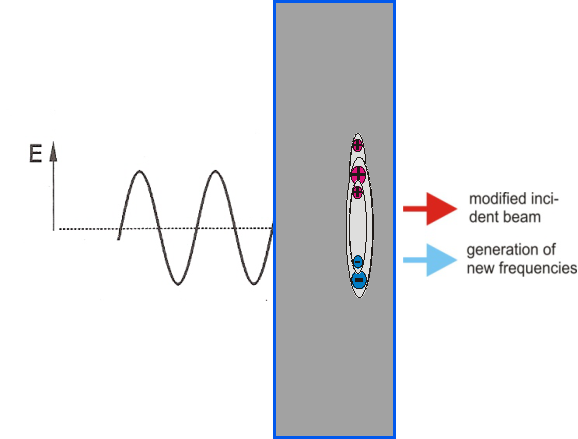
\includegraphics[width=\columnwidth]{inducedDipole2}
      \caption{Induced dipole}
      \label{fig:indDipole}
    \end{figure}


  \end{columns}
\end{frame}



%%% Local Variables: 
%%% mode: latex
%%% TeX-master: "nonlinearslides"
%%% TeX-engine: default
%%% End: 
